\documentclass[aspectratio=169, 11pt]{beamer}

% --- Packages & Setup ---
\usepackage[utf8]{inputenc}
\usepackage[T1]{fontenc}
\usepackage{amsmath}
\usepackage{amssymb}
\usepackage{textcomp}
\usepackage{xcolor}
\usepackage{booktabs}
\usepackage{graphicx}
\usepackage{tabularx}
\usepackage{tikz}
\usetikzlibrary{calc,positioning,arrows.meta}
\usepackage{url}
\usepackage{multirow}
\usepackage{float}

\graphicspath{{../}{./}}

\IfFileExists{opensans.sty}{\usepackage[default,scale=0.95]{opensans}}{}

\newcommand{\safefig}[2][width=0.6\linewidth]{%
  \IfFileExists{#2}%
    {\includegraphics[#1]{#2}}%
    {\fbox{\parbox[c][1.4cm][c]{3.8cm}{\centering\tiny
      \textit{Missing:}\\ \texttt{\detokenize{#2}}}}}%
}

% --- Branding Colors ---
\definecolor{amritaMaroon}{HTML}{A4123F}

% --- Theme Setup ---
\usetheme{Madrid}
\usecolortheme[named=amritaMaroon]{structure}
\setbeamertemplate{navigation symbols}{}
\setbeamertemplate{footline}[frame number]
\setbeamertemplate{bibliography item}[text]

\begin{document}

% ============================================================
% TITLE SLIDE
% ============================================================
\begin{frame}
    \begin{tikzpicture}[remember picture,overlay]
        \node[fill=amritaMaroon, text=white, font=\bfseries\footnotesize,
              anchor=north east, rounded corners=2pt, inner sep=5pt]
        at ($(current page.north east) + (-0.2cm,-0.2cm)$)
        {Type 1: Research Project};
    \end{tikzpicture}

    \centering
    \safefig[width=2.8cm]{logo.png}
    \vspace{0.1cm}

    {\large \textbf{\textcolor{amritaMaroon}{%
        Climate-Adaptive Intelligent Control and Optimization of
        PCM Thermal Storage for Solar Water Heating%
    }}}\\
    \vspace{0.05cm}
    {\footnotesize \textbf{23CSE498 --- Project Phase 2 (Panel Review 2)}
    \quad|\quad \textbf{Group 12}}\\
    \vspace{0.15cm}

    \begin{table}
        \centering
        \footnotesize
        \renewcommand{\arraystretch}{1.05}
        \begin{tabular}{|c|c|l|}
            \hline
            \textbf{S.No} & \textbf{Register Number} & \textbf{Student Name} \\
            \hline
            1 & CB.SC.U4CSE23430 & MANDUVA JASWITA \\
            \hline
            2 & CB.SC.U4CSE23318 & DUNGI MANVITHA \\
            \hline
            3 & CB.SC.U4CSE23412 & DUDDEKUNTA YUVA HASINI \\
            \hline
            4 & CB.SC.U4CSE23558 & CHIRUVOLU VENKATA KHYATHI \\
            \hline
            5 & CB.SC.U4CSE23034 & K P N L K MAHITHA \\
            \hline
        \end{tabular}
    \end{table}
    \vspace{0.1cm}

    {\footnotesize Guide: \textbf{Dr.\ T.\ Deepika},
     \textbf{Assistant Professor (Sr.\ Gd.)}, Department of CSE}\\
    \vspace{0.1cm}
    {\scriptsize \today}
\end{frame}

% ============================================================
% TABLE OF CONTENTS
% ============================================================
\begin{frame}{Table of Contents}
\begin{enumerate}
    \item Motivation
    \item Research Gaps \& Problem Statement
    \item Objectives
    \item Methodology \& Solution Design
    \item Implementation Progress
    \item Technical Knowledge \& Design Decisions
    \item Technical Enrichment Activity
    \item References
\end{enumerate}
\end{frame}

% ============================================================
% SECTION 1: INTRODUCTION & MOTIVATION
% ============================================================
\section{Introduction \& Motivation}

\begin{frame}{1. Motivation}
\begin{itemize}
    \item Thermal energy accounts for 48--50\% of global final energy consumption. Residential water heating uses 6--8\% of household energy, underscoring SWH potential \cite{AlMamun2023SWHReview}.
    \item Conventional solar water heating (SWH) systems achieve only 45--70\% annual efficiency, wasting 30--55\% of incident solar energy due to inadequate storage \cite{AlMamun2023SWHReview}.
    \item PCM-integrated systems can boost thermal efficiency, extend heat retention time and store $\sim$50\% of total heat with $<$20\% PCM volume \cite{Singh2025PCMSWH, Hamza2025PCMReview, Rathore2024ThermalPCM}.
    \item Global solar thermal capacity reaches $\sim$544--560 GW$_{th}$ (2024--2025); The global market for water heaters was valued at \$23.7 billion as of 2023. It is expected to reach \$32.1 billion by 2029 \cite{OdoiYorke2025AI_SWH}.
    \item Existing PCM-SWH systems use mostly fixed/offline strategies, causing losses under variable irradiance/load; this motivates our adaptive-control approach \cite{Barqawi2025MLPCMSWH, Emami2026DRLSolar}.
\end{itemize}
\end{frame}

% ============================================================
% SECTION 2: RESEARCH GAPS & PROBLEM STATEMENT
% ============================================================
\section{Research Gaps \& Problem Statement}

\begin{frame}{2.1 Research Gaps}
\small
\begin{enumerate}
    \item \textbf{Limited real-time adaptive control:}
    Most PCM-based systems use passive or fixed-rule strategies, lacking dynamic response to varying solar input and demand \cite{Barqawi2025MLPCMSWH, Emami2026DRLSolar}.
    \item \textbf{Lack of integrated PCM--AI--hardware systems:}
    Prior studies treat materials, control, and implementation separately without a complete working prototype \cite{OdoiYorke2025AI_SWH, Liu2025AIPCM}.
    \item \textbf{Poor alignment with real usage patterns:}
    Existing systems rarely adapt storage and release based on actual household demand \cite{Assareh2023ML_PCM_SolarCollector}.
    \item \textbf{Limited real-world validation:}
    Most research relies on simulations or short-term tests rather than long-term experimental evaluation \cite{Chopra2023MonteCarloETC, Duraivel2025DSTS}.
    \item \textbf{Limited predictive optimization under climatic uncertainty:}
    Most PCM-based systems lack predictive models to anticipate variations in solar input and demand, leading to suboptimal thermal storage utilization \cite{Ghodusinejad2026SolarForecast, Mohammed2025AIthermal}.
\end{enumerate}
\end{frame}

\begin{frame}{2.2 Problem Statement}
\vspace{0.3cm}
\begin{block}{Novel Idea}
To design and implement an autonomous, AI-driven PCM-based thermal storage system that dynamically optimizes heat charging and discharging under real-world operating conditions \cite{Liu2025AIPCM, Emami2026DRLSolar}.
\end{block}

\vspace{0.4cm}
\textbf{Sustainable Development Goals related to the problem:}
\vspace{0.3cm}
\begin{center}
\begin{tabular}{c c c c}
\safefig[width=2.2cm]{7.png} &
\safefig[width=2.2cm]{9.png} &
\safefig[width=2.2cm]{12.png} &
\safefig[width=2.2cm]{13.png}
\end{tabular}
\end{center}
\end{frame}

% ============================================================
% SECTION 3: OBJECTIVES
% ============================================================
\section{Objectives}

\begin{frame}{3.1 Objectives}
\begin{block}{Overall Problem}
Most PCM-based solar water heating systems use passive or fixed control rules,
leading to delayed heat availability, inefficient storage, and energy loss
under variable climatic and hot-water demand conditions \cite{Barqawi2025MLPCMSWH}.
\end{block}

\footnotesize
\begin{itemize}
\item \textbf{Objective 1 (O1):} Develop a climate-region-aware recommendation framework that clusters large-scale meteorological data and identifies the Top-2/Top-3 suitable PCM candidates for different climatic conditions using multi-criteria decision-making \cite{Singh2025PCMSWH, Hamza2025PCMReview, Ghodusinejad2026SolarForecast}.

\item \textbf{Objective 2 (O2):} Develop an AI-driven design optimization model to determine the optimal PCM thickness, capsule arrangement, number of PCM capsules, and flow rate for maximizing thermal energy storage under location-specific climatic conditions \cite{Chen2025TaguchiGRAPCM, Barqawi2025MLPCMSWH, Kou2025BIHPPCM}.

\item \textbf{Objective 3 (O3):} Design a Deep Reinforcement Learning (DRL)-based adaptive controller to optimize PCM charging, discharging, and bypass operations under dynamic weather and hot-water demand \cite{Emami2026DRLSolar, Sivaraj2023DRLShip}.

\item \textbf{Objective 4 (O4):} Deploy and validate the intelligent PCM management framework on embedded hardware under representative Indian climatic regions to evaluate thermal efficiency, energy savings, and operational reliability \cite{Duraivel2025DSTS, Chopra2023MonteCarloETC}.
\end{itemize}
\end{frame}

% ------------------------------------------------------------
% 3.2 O1 Architecture (moved from old 4.1)
% ------------------------------------------------------------
\begin{frame}{3.2 Architecture Diagram}
    \begin{figure}
        \centering
        \safefig[width=1\textwidth,height=0.9\textheight,keepaspectratio]{obj_overall.png}
    \end{figure}
\end{frame}

% ============================================================
% SECTION 4: METHODOLOGY & SOLUTION DESIGN
% ============================================================
% NOTE: Objective 1 (O1) content below has been reorganized into a single
% continuous workflow (4.1 -- 4.13) per panel-review request. Objective 2
% content (design optimization) previously interleaved in this section has
% been left untouched in its own frames further below / in Section 6, per
% the "do not touch O2/O3/O4" instruction.
\section{Methodology \& Solution Design}

% ------------------------------------------------------------
% 4.1 Objective 1 (restated, scoped)
% ------------------------------------------------------------
\begin{frame}{4.1 Objective 1 --- Climate-Region-Aware PCM Recommendation}
\begin{block}{Objective 1 (O1)}
Develop a climate-region-aware recommendation framework that clusters
large-scale meteorological data and identifies the Top-2/Top-3 suitable
PCM candidates for different climatic conditions using multi-criteria
decision-making.
\end{block}

\vspace{0.3cm}
\textbf{O1 story, at a glance:}
\begin{itemize}\small
    \item Collect and clean multi-year climate data across four Indian states \cite{Hersbach2020Era5, Stackhouse2021POWER}
    \item Identify climate regimes via clustering
    \item Screen and rank PCM candidates for each regime using MCDM \cite{Singh2025PCMSWH}
    \item Validate the MCDM ranking against physics-based simulation \cite{Barqawi2025PCMSim}
    \item Recommend Top PCM candidates per climate regime
\end{itemize}
\end{frame}

% ------------------------------------------------------------
% 4.2 O1 Architecture (moved from old 4.1)
% ------------------------------------------------------------
\begin{frame}{4.2 Objective 1 Architecture}
    \begin{figure}
        \centering
        \safefig[width=1\textwidth,height=0.9\textheight,keepaspectratio]{Objective1.drawio (1).png}
    \end{figure}
\end{frame}

% ------------------------------------------------------------
% 4.3 Dataset & Spatial Sampling
% (merged: old 4.3 dataset bullets + old 4.4 ERA5/NASA POWER variable table,
%  condensed into grouped categories + old 4.5 data collection point maps)
% ------------------------------------------------------------
\begin{frame}{4.3 Dataset \& Spatial Sampling}
\framesubtitle{ERA5 + NASA POWER hourly reanalysis across 4 Indian climate regions}

\begin{columns}[T]
    \column{0.52\textwidth}
    \small
    \textbf{Data sources}
    \begin{itemize}\footnotesize
        \item \textbf{ERA5}~\cite{Hersbach2020Era5} --- primary hourly reanalysis dataset
        \item \textbf{NASA POWER}~\cite{Stackhouse2021POWER} --- independent cross-check dataset
        \item Hourly temporal resolution
        \item Population-weighted spatial grid sampling~\cite{Stevens2015WorldPop}
        \item \textbf{Four study states:} Assam, Rajasthan, Tamil Nadu, Uttarakhand
    \end{itemize}

    \vspace{0.15cm}
    \textbf{Climate variables (grouped)}
    \begin{itemize}\footnotesize
        \item \textbf{Solar/radiation:} GHI, DNI, DHI, clear-sky GHI, clearness index, solar zenith \& azimuth angle \cite{RedaAndreas2004SPA, IneichenPerez2002ClearSky}
        \item \textbf{Thermal/humidity:} ambient temperature, dewpoint temperature, relative humidity \cite{Alduchov1996Magnus}
        \item \textbf{Atmospheric:} wind speed, wind direction, surface pressure, cloud cover, precipitation
    \end{itemize}
    {\tiny NASA POWER used for independent cross-check of GHI, clear-sky GHI, ambient temperature, relative humidity, and wind speed at 10\,m \cite{Stackhouse2021POWER}.}

    \column{0.48\textwidth}
    \centering
    \includegraphics[width=0.95\linewidth, height=0.38\textheight]{rj_a_point.png}\\[0.05cm]
    \includegraphics[width=0.95\linewidth, height=0.38\textheight]{tn_A_point_map.png}
    {\tiny ERA5 grid point distribution (sample states shown)}
\end{columns}
\end{frame}

% ------------------------------------------------------------
% 4.4 Data Preprocessing & Quality Control
% (merged: old 4.3 QC bullet + old 4.6 raw-vs-preprocessed plots +
%  old 4.7 preprocessing summary plots + relevant part of old 5.2 module row)
% ------------------------------------------------------------
\begin{frame}{4.4 Data Preprocessing \& Quality Control}
\framesubtitle{Raw data $\to$ QC $\to$ bias correction $\to$ compressed climate signature}

\begin{columns}[T]
    \column{0.42\textwidth}
    \small
    \textbf{Preprocessing workflow}
    \begin{itemize}\footnotesize
        \item Raw ERA5/NASA POWER data
        \item Unit conversion (e.g.\ K$\to^\circ$C, flux conversions)
        \item Outlier detection/treatment: \textbf{Hampel/MAD filter}~\cite{Hampel1974InfluenceCurve}
        \item Missing-value treatment: \textbf{MICE imputation}~\cite{Rubin1987MultipleImputation, vanBuuren2011MICE}
        \item Bias correction: \textbf{quantile mapping} (per-season)~\cite{Themessl2012QM}
        \item Dimensionality reduction: \textbf{PCA}-compressed climate signature
    \end{itemize}

    \column{0.58\textwidth}
    \centering
    \includegraphics[width=0.48\linewidth, height=0.28\textheight]{am_01_raw_vs_preprocessed_radiation.png}\hfill
    \includegraphics[width=0.48\linewidth, height=0.28\textheight]{rj_1_raw_vs_preprocessed_radiation.png}\\[0.1cm]
    \includegraphics[width=0.48\linewidth, height=0.28\textheight]{tn_01_raw_vs_preprocessed_radiation.png}\hfill
    \includegraphics[width=0.48\linewidth, height=0.28\textheight]{uk_01_raw_vs_preprocessed_radiation.jpeg}\\[0.05cm]
    {raw vs.\ preprocessed radiation.}
\end{columns}
\end{frame}

% ------------------------------------------------------------
% 4.5 Climate Signature & Clustering (moved from old 5.3, with explanation)
% ------------------------------------------------------------
\begin{frame}{4.5 Climate Signature \& Clustering}
\framesubtitle{Grouping locations into climate regimes for region-specific PCM recommendation}

\footnotesize
Locations with similar climatic behavior are grouped into climate regimes
so that PCM recommendations are climate-region specific \cite{FraleyRaftery2007ModelBased, McLachlanPeel2000FMM}.

% RESOLVED: State-wise cluster counts below are now confirmed from source
% data (mcdm_topk_by_cluster.csv / mcdm_topk_assam.csv / audit docs), not
% invented. The earlier uniform "K=5" description elsewhere in this deck
% (Sec. 5, module-functionality table) refers to one implementation
% description only; actual per-state K differs as shown below.
\textbf{State-wise cluster count (GMM, BIC + silhouette):}\quad
Assam: 3 \quad|\quad
Rajasthan: 3 \quad|\quad
Tamil Nadu: 5 \quad|\quad
Uttarakhand: 5

\vspace{0.15cm}
\centering
\begin{tabular}{cccc}
\includegraphics[width=0.235\linewidth,height=0.42\textheight,keepaspectratio]{am_04_geographic_map.png} &
\includegraphics[width=0.235\linewidth,height=0.42\textheight,keepaspectratio]{rj_04_geographic_map.png} &
\includegraphics[width=0.235\linewidth,height=0.42\textheight,keepaspectratio]{tn_04_geographic_map.png} &
\includegraphics[width=0.235\linewidth,height=0.42\textheight,keepaspectratio]{uk_04_geographic_map.png} \\
{\tiny Assam} & {\tiny Rajasthan} & {\tiny Tamil Nadu} & {\tiny Uttarakhand}
\end{tabular}
\end{frame}


% ------------------------------------------------------------
% 4.6 Multi-Method MCDM Ranking
% ------------------------------------------------------------
\begin{frame}{4.6 Multi-Method MCDM Ranking}
\framesubtitle{Ranking pipeline overview (see 4.8 for method-selection rationale)}
\vspace{-0.3cm}
\begin{center}
\scalebox{0.8}{
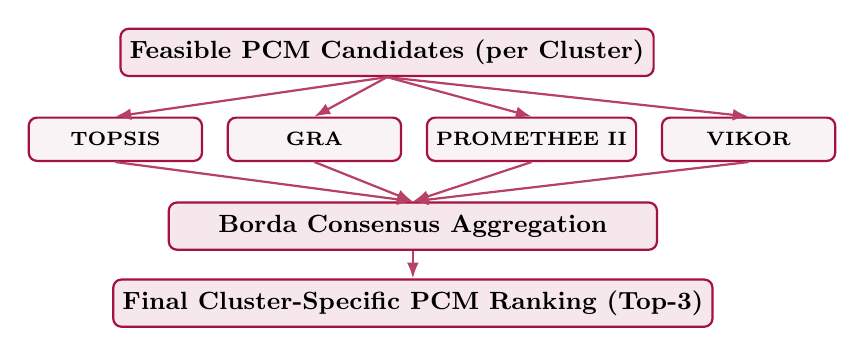
\begin{tikzpicture}[
    box/.style={draw=amritaMaroon, thick, rounded corners=3pt, fill=amritaMaroon!10, minimum width=6.2cm, minimum height=0.6cm, align=center, font=\small\bfseries},
    smallbox/.style={draw=amritaMaroon, thick, rounded corners=3pt, fill=amritaMaroon!5, minimum width=2.2cm, minimum height=0.55cm, align=center, font=\scriptsize\bfseries},
    arr/.style={-{Latex[length=2mm, width=1.5mm]}, thick, draw=amritaMaroon!80}
]
% Nodes
\node[box] (feas) {Feasible PCM Candidates (per Cluster)};
\node[smallbox, below=0.5cm of feas, xshift=-3.45cm] (topsis) {TOPSIS};
\node[smallbox, right=0.3cm of topsis] (gra) {GRA};
\node[smallbox, right=0.3cm of gra] (prom) {PROMETHEE II};
\node[smallbox, right=0.3cm of prom] (vikor) {VIKOR};
\node[box, below=0.5cm of gra, xshift=1.25cm] (borda) {Borda Consensus Aggregation};
\node[box, below=0.35cm of borda] (final) {Final Cluster-Specific PCM Ranking (Top-3)};
% Arrows
\draw[arr] (feas.south) -- (topsis.north);
\draw[arr] (feas.south) -- (gra.north);
\draw[arr] (feas.south) -- (prom.north);
\draw[arr] (feas.south) -- (vikor.north);
\draw[arr] (topsis.south) -- (borda.north);
\draw[arr] (gra.south) -- (borda.north);
\draw[arr] (prom.south) -- (borda.north);
\draw[arr] (vikor.south) -- (borda.north);
\draw[arr] (borda.south) -- (final.north);
\end{tikzpicture}}
\end{center}
\vspace{-0.15cm}
\begin{block}{\scriptsize Multi-Criteria Evaluation Pipeline}
\begin{itemize}\scriptsize
    \setlength{\itemsep}{0pt}
    \item \textbf{Harmonized Inputs:} All 4 methods evaluate the \emph{identical} feasible candidate pool using the \emph{same} 5 criteria and a unified 50\% Shannon entropy + 50\% AHP blended weight vector \cite{Saaty1980AHP}.
    \item \textbf{Decision Criteria (Benefit):} Melting-point fitness ($f_{T_m}$, Gaussian target proximity), latent heat ($L$), volumetric storage density ($\rho L$), thermal conductivity ($k$), and cycling endurance \cite{Singh2025PCMSWH, Hamza2025PCMReview}.
    \item \textbf{Method origins:} GRA~\cite{Deng1982GreySystems}, PROMETHEE~II~\cite{BransMareschal2005PROMETHEE}, VIKOR~\cite{OpricovicTzeng2004VIKOR}.
    \item \textbf{Borda Consensus:} Aggregates individual method ranks into a robust consensus rank sum: $\text{Score}_i = \sum_{m=1}^{4} (N - \text{rank}_{m,i} + 1)$, mitigating single-method mathematical bias.
    \item \textbf{Regime-Specific Output:} Generates definitive Top-1 and Top-3 recommendations tailored to the thermal load and solar availability of each climate cluster.
\end{itemize}
\end{block}
\end{frame}

% ------------------------------------------------------------
% 4.7 Technical Knowledge -- Four MCDM Methods Overview
% (RENUMBERED from old mislabeled "4.8"; placed directly after the
%  4.6 pipeline diagram, ahead of the "why four methods" rationale slide,
%  since a reviewer needs to see what each method IS before reading why
%  all four were used together)
% ------------------------------------------------------------
\begin{frame}{4.7 Technical Knowledge --- Four MCDM Methods Overview}
\framesubtitle{Rubric: Core MCDM algorithms for O1 PCM recommendation}

\begin{columns}[T]
    \column{0.5\textwidth}
    \small
    \textbf{1. TOPSIS}
    \begin{itemize}
        \item Ranks PCM from our 8 criteria (latent heat, $\rho L$, conductivity, cycling stability, supercooling, corrosion, cost, melting-point fitness).
        \item it's a geometric closeness score $C_i$, not a rule-based score
    \end{itemize}

    \vspace{0.15cm}
    \textbf{2. PROMETHEE II}~\cite{BransMareschal2005PROMETHEE}
    \begin{itemize}
        \item Compares every pair of PCMs, using a preference function.
        \item Sums up how often/how strongly each PCM ``beats'' every other PCM into a net flow $\phi$ --- ranking by outranking strength, not distance
    \end{itemize}

    \column{0.5\textwidth}
    \small
    \textbf{3. GRA (Grey Relational Analysis)}~\cite{Deng1982GreySystems}
    \begin{itemize}
        \item Treats the best value of each criterion as a reference, then measures how closely each real PCM ``tracks'' that reference curve.
        \item Ranking is by grey relational grade $\Gamma \in [0,1]$: higher means the PCM's overall property pattern shadows the ideal pattern.
    \end{itemize}

    \vspace{0.15cm}
    \textbf{4. VIKOR}~\cite{OpricovicTzeng2004VIKOR}
    \begin{itemize}
        \item Computes two separate scores : $S_i$ (how far it is from ideal \emph{averaged} across all 8 criteria) and $R_i$ (its \emph{single worst} criterion gap)
        \item VIKOR sometimes disagrees sharply with TOPSIS on a PCM that's good on average but weak on one criterion (e.g.\ cost)
    \end{itemize}
\end{columns}
\end{frame}
% ------------------------------------------------------------
% 4.8 Why Four MCDM Methods?
% (RENUMBERED from old 4.7; content unchanged -- moved/condensed from old
%  6.3, left column only. Now follows the methods-overview slide instead
%  of preceding it.)
% ------------------------------------------------------------
\begin{frame}{4.8 Why Four MCDM Methods?}
\small
\begin{itemize}
    \item \textbf{Avoid single-method artifacts:} each method's underlying math can bias a ranking; using one method risks hidden assumptions driving the result \cite{Figueira2005MCDA}.
    \item \textbf{Different methods can disagree:} TOPSIS, GRA~\cite{Deng1982GreySystems}, PROMETHEE~II~\cite{BransMareschal2005PROMETHEE} and VIKOR~\cite{OpricovicTzeng2004VIKOR} use different distance/preference logics and can rank PCMs differently for the same data.
    \item \textbf{Consensus reduces single-method dependence:} \textbf{Borda aggregation} combines the four rankings into one consensus ranking.
    \item \textbf{Agreement check:} \textbf{Kendall's $W$} measures inter-method agreement ($W \to 1$ indicates strong consensus).
    \item Disagreement between methods is treated as a signal of criterion sensitivity, not simply averaged away.
\end{itemize}
\end{frame}

% ------------------------------------------------------------
% 4.9 PCM Rank Evolution
% (RENUMBERED from old mislabeled "4.11"; moved from old 5.5. Now placed
%  right after the method-selection rationale so the reader sees how ranks
%  evolve across the four MCDM methods before the stability/physics checks.)
% ------------------------------------------------------------
\begin{frame}{4.9 PCM Rank Evolution}
\framesubtitle{MCDM ranking: PCM rank evolution across all 4 states}
\vspace{0.05cm}
\centering
\setlength{\tabcolsep}{2pt}
\begin{tabular}{cc}
\includegraphics[width=0.47\linewidth,height=0.35\textheight,keepaspectratio]{am_0_bump_chart.png} &
\includegraphics[width=0.47\linewidth,height=0.35\textheight,keepaspectratio]{rj_0_bump_chart.png} \\
{\tiny Assam} & {\tiny Rajasthan} \\[0.06cm]
\includegraphics[width=0.5\linewidth,height=0.37\textheight,keepaspectratio]{tn_0_bump_chart.png} &
\includegraphics[width=0.5\linewidth,height=0.37\textheight,keepaspectratio]{uk_0_bump_chart.jpeg} \\
{\tiny Tamil Nadu} & {\tiny Uttarakhand}
\end{tabular}
\end{frame}

% ------------------------------------------------------------
% 4.10 Ranking Stability -- 5000 Monte Carlo Runs
% (RENUMBERED from old mislabeled "4.8" (the Monte Carlo frame, not the
%  MCDM-methods-overview frame that also incorrectly used "4.8"). Content
%  unchanged.)
% ------------------------------------------------------------
\begin{frame}{4.10 Ranking Stability --- 5000 Monte Carlo Runs}
\framesubtitle{Testing whether the consensus ranking holds under uncertainty}

\footnotesize
MCDM weights + PCM property uncertainty $\to$ random perturbation $\to$ ranking runs $\to$ Top-3 inclusion probability \cite{Chopra2023MonteCarloETC}

\vspace{0.15cm}
\textbf{Monte Carlo Ranking Stability (Top-1 Consensus Winners):}
\vspace{0.1cm}

\begin{table}[H]
\centering
\scriptsize
\setlength{\tabcolsep}{4pt}
\renewcommand{\arraystretch}{1.15}
\begin{tabular}{llccc}
\hline
\textbf{Region (Draws)} & \textbf{Climate Regime / Cluster} & \textbf{Rank-1 PCM} & \textbf{Top-3 Incl.} & \textbf{Top-1 Ret.} \\
\hline
\textbf{Assam} & Cluster 0 (Lower Brahmaputra) & RT44HC & \textbf{96.2\%} & 66.7\% \\
(5,000 draws)  & Cluster 1 (Upper Assam)       & RT44HC & \textbf{95.5\%} & 59.8\% \\
               & Cluster 2 (Barak Valley)      & RT44HC & \textbf{95.3\%} & 59.8\% \\
\hline
\textbf{Rajasthan} & Cluster 0 (Southern Plateau)  & savE\textregistered{} OM55  & \textbf{99.9\%} & 67.6\% \\
(1,000 draws)      & Cluster 1 (Thar Arid Core)    & PureTemp 60                  & \textbf{99.3\%} & 78.1\% \\
                   & Cluster 2 (Shekhawati)        & n-Heptacosane (C27)          & \textbf{91.6\%} & 55.1\% \\
\hline
\textbf{Tamil Nadu} & Clusters 0, 2, 3 (Inland/Delta/Plains) & n-Octacosane & \textbf{76.8--77.8\%} & 50.8--51.2\% \\
(5,000 draws)       & Clusters 1, 4 (Western/Coastal)       & n-Octacosane & \textbf{90.2\%}       & 71.0\% \\
\hline
\textbf{Uttarakhand (5,000 draws)} & Clusters 0--4 (Himalayan Regimes) & n-Octacosane (C28) & \textbf{37.8--39.3\%} & 16.2--18.3\% \\
\hline
\end{tabular}
\end{table}

\end{frame}

% ------------------------------------------------------------
% 4.11 Physics-Based Validation (Lumped-Enthalpy Model)
% UPDATED: Spearman rank-correlation formula/interpretation removed
% (correlation sign varies by state/cluster). Thermal balance equation
% kept but given a plain-language reading so it is easier to narrate
% live. Enthalpy-temperature relation kept as-is.
% ------------------------------------------------------------
\begin{frame}{4.11 Physics-Based Validation (Lumped-Enthalpy Model)}
\framesubtitle{Why and how physics-based validation is performed}

\footnotesize
\textbf{Motivation:} MCDM provides a static ranking. Physics simulation
checks whether that ranking is supported by dynamic thermal behavior \cite{Barqawi2025PCMSim, Abdellatif2025PCM_Modeling}.

\vspace{0.15cm}
\textbf{Thermal Energy Balance (lumped-enthalpy model)}~\cite{Barqawi2025PCMSim, MADADIAVARGANI2021101350}:
\[
m_{\mathrm{PCM}}\frac{dH}{dt} = \dot{Q}_{\mathrm{solar}} - UA(T-T_{\mathrm{amb}}) - \dot{Q}_{\mathrm{draw}}
\]
\textit{In words:} rate of PCM energy storage = solar gain
$-$ heat lost to ambient $-$ heat removed by hot-water draw.

\vspace{0.1cm}
\begin{columns}[T]
    \column{0.5\textwidth}
    \footnotesize
    \begin{itemize}
        \setlength{\itemsep}{0pt}
        \item $m_{\mathrm{PCM}}$ = PCM mass (kg)
        \item $\dot{Q}_{\mathrm{solar}}$ = solar heat input (W)
        \item $UA$ = tank heat loss coeff. (W/K)
        \item $\dot{Q}_{\mathrm{draw}}$ = hot-water draw (W)
    \end{itemize}

    \column{0.5\textwidth}
    \small
    \textbf{Enthalpy-Temperature Relation}~\cite{Abdellatif2025PCM_Modeling}:
    \footnotesize
    \[
    H(T) = \begin{cases}
    c_{s}\,T & T < T_{m} \text{ (solid)} \\
    L + c_{l}\,T & T > T_{m} \text{ (liquid)}
    \end{cases}
    \]
    \begin{itemize}
        \setlength{\itemsep}{0pt}
        \item $L$ = latent heat of fusion (J/kg)
        \item $c_s, c_l$ = specific heats (J/kg·K)
        \item $T_m$ = melting point (°C)
    \end{itemize}
\end{columns}
\end{frame}


% ------------------------------------------------------------
% 4.12 MCDM vs Physics Ranking
% (RENUMBERED from old 4.10; moved from old 5.4. Content unchanged.)
% ------------------------------------------------------------
\begin{frame}{4.12 MCDM vs Physics Ranking}
\framesubtitle{Inter-method / physics agreement across all 4 states}

\scriptsize
x-axis = simulation rank \quad|\quad y-axis = MCDM consensus rank \quad|\quad
$y=x$ = perfect agreement \quad|\quad color = climate cluster

\vspace{0.05cm}
\centering
\setlength{\tabcolsep}{2pt}
\begin{tabular}{cc}
\includegraphics[width=0.55\linewidth,height=0.35\textheight,keepaspectratio]{am_agreement_plot.png} &
\includegraphics[width=0.55\linewidth,height=0.35\textheight,keepaspectratio]{rj_agreement_plot.png} \\
{\tiny Assam} & {\tiny Rajasthan} \\[0.03cm]
\includegraphics[width=0.55\linewidth,height=0.35\textheight,keepaspectratio]{tn_11_agreement_plot.png} &
\includegraphics[width=0.55\linewidth,height=0.35\textheight,keepaspectratio]{uk_11_agreement_plot.jpeg} \\
{\tiny Tamil Nadu} & {\tiny Uttarakhand}
\end{tabular}
\end{frame}


% ------------------------------------------------------------
% 4.13 Objective 1 -- Final PCM Recommendations
% ------------------------------------------------------------
\begin{frame}{4.13 Objective 1 --- Final PCM Recommendations}
\framesubtitle{Consolidated Top-3 PCM recommendation per climate regime}

\tiny
\begin{table}
\centering
\renewcommand{\arraystretch}{1.15}
\resizebox{\textwidth}{!}{
\begin{tabular}{l l l l l}
\toprule
\textbf{State} & \textbf{Climate Cluster} & \textbf{Top-1 PCM} & \textbf{Top-2 PCM} & \textbf{Top-3 PCM} \\
\midrule
\multirow{5}{*}{Tamil Nadu}
 & 0 (Coastal Plain / Chennai) & n-Octacosane (C28) & n-Hexacosane (C26) & PureTemp 58 \\
 & 1 (Inland Plains / Salem--Coimbatore) & n-Octacosane (C28) & RT64HC & n-Hexacosane (C26) \\
 & 2 (Cauvery Delta / Central Agro-Belt) & n-Octacosane (C28) & PureTemp 58 & n-Hexacosane (C26) \\
 & 3 (Southern Dry Zone / Madurai) & n-Octacosane (C28) & PureTemp 58 & n-Hexacosane (C26) \\
 & 4 (Western Ghats / Nilgiris) & n-Octacosane (C28) & RT64HC & n-Hexacosane (C26) \\
\midrule
\multirow{3}{*}{Rajasthan}
 & 0 (Southern Plateau / Udaipur--Kota) & savE\textregistered{} OM55 & Palmitic-stearic acid/EG & Myristic acid/NBR-0.5 \\
 & 1 (Thar Arid Core / Jaisalmer--Jodhpur) & PureTemp 60 & CrodaTherm 60 & n-Heptacosane (C27) \\
 & 2 (NE Shekhawati / Jaipur--Bikaner) & n-Heptacosane (C27) & PureTemp 58 & PlusICE A58 \\
\midrule
\multirow{3}{*}{Assam}
 & 0 (Lower Brahmaputra Valley / Guwahati) & RT44HC & RT45HC & C22H46 (n-Docosane) \\
 & 1 (Upper Assam Tea Belt / Dibrugarh--Jorhat) & RT44HC & RT45HC & C22H46 (n-Docosane) \\
 & 2 (Barak Valley \& Foothills / Silchar) & RT44HC & RT45HC & RT54HC \\
\midrule
\multirow{5}{*}{Uttarakhand}
 & 0 (Siwalik/Bhabar Transition, ~740m) & PureTemp 58 & n-Octacosane (C28) & PlusICE A58 \\
 & 1 (High Himalaya / Alpine, ~2220m) & PureTemp 53 & n-Hexacosane (C26) & Myristic acid (C14) \\
 & 2 (Western Garhwal Mid-Hills, ~1300m) & PureTemp 58 & savE\textregistered{} OM55 & n-Hexacosane (C26) \\
 & 3 (Tarai-Bhabar Plains / Haridwar--Dehradun, ~320m) & PureTemp 58 & savE\textregistered{} OM55 & Palmitic-stearic/EG \\
 & 4 (Kumaon Mid-Hills / Nainital--Almora, ~1450m) & PureTemp 58 & n-Octacosane (C28) & PlusICE A58 \\
\bottomrule
\end{tabular}
}
\end{table}

\vspace{0.05cm}
\end{frame}

% ------------------------------------------------------------
% 4.14 From Objective 1 to Objective 2
% NEW SLIDE: bridges the O1 outputs (4.9-4.13)
% content and the O2 story already on 5.1 -- no new claims introduced.
% ------------------------------------------------------------
\begin{frame}{Bridging Objective 1 and Objective 2}
\framesubtitle{A smooth transition from analysis to design}

\footnotesize
\begin{itemize}
    \setlength{\itemsep}{6pt}
    \item Objective 1 successfully mapped the climate conditions across
    all four states, giving a clear picture of what each region needs.
    \item For every climate zone, the best-suited PCM candidates were
    successfully identified and shortlisted.
    \item These results were thoroughly validated, confirming that the
    findings are reliable and ready to be used further.
    \item This solid foundation now carries forward directly into
    Objective 2, where the shortlisted materials are further refined
    and optimized for real-world performance.
\end{itemize}
\end{frame}


% ============================================================
% OBJECTIVE 2 SLIDES -- replaces old frames 5.6, 5.8, and 6.2
% Insert this block immediately after "5.1 Implementation Progress
% --- Overall Status" and before "5.9"/whatever the next surviving
% frame is. Also delete the now-empty \section{Technical Knowledge}
% line, since 6.2 was its only frame.
%
% Numbering follows the Objective 1 template (4.1 restated-objective
% + "story at a glance" -> 4.2 architecture placeholder -> detail
% slides -> key findings), renumbered into the 5.x Implementation
% Progress sequence since that is where Objective 2 already lives
% in this deck. Renumber freely if you'd rather it sit elsewhere.
% ============================================================

% ------------------------------------------------------------
% 5.2 Objective 2 (restated, scoped) -- mirrors 4.1
% ------------------------------------------------------------
% ============================================================
% OBJECTIVE 2 SLIDES (v2 -- with plots) -- replaces old frames
% 5.6, 5.8, and 6.2. Also delete the now-empty
% \section{Technical Knowledge} line, since 6.2 was its only frame.
%
% Image filenames follow the Objective 1 convention (state-prefixed:
% tn_, rj_, am_, uk_) so the four-state grids look consistent with
% 4.5/4.9/4.12. Your actual plot files (from make_plots.py) are NOT
% state-prefixed by default -- e.g. results/tamilnadu/plots/static/
% phase4_gate3_baseline_comparison.png -- so copy/rename one per
% state before compiling, e.g.:
%   cp results/tamilnadu/plots/static/phase4_gate3_baseline_comparison.png ./tn_phase4_gate3_baseline_comparison.png
%   cp results/rajasthan/plots/static/phase4_gate3_baseline_comparison.png ./rj_phase4_gate3_baseline_comparison.png
%   ... etc for am_, uk_
% Do the same for the feature-importance, Pareto, and robustness
% plots referenced below. If a state's plot isn't ready yet, safefig
% will render a "Missing: <filename>" placeholder box instead of
% crashing the build.
% ============================================================

% ------------------------------------------------------------
% 5.2 Objective 2 (restated, scoped) -- mirrors 4.1
% ------------------------------------------------------------
\begin{frame}{5.1 Objective 2 --- AI-Driven Design Optimization}
\begin{block}{Objective 2 (O2)}
Develop an AI-driven design optimization model to determine the optimal
PCM thickness, capsule arrangement, number of PCM capsules, and flow
rate for maximizing thermal energy storage under location-specific
climatic conditions.
\end{block}

\vspace{0.3cm}
\textbf{O2 story, at a glance:}
\begin{itemize}\small
    \item Freeze a shared collector/tank/safety configuration across all
    states, so climate is the only variable that changes
    \cite{Singh2025PCMSWH, Chen2025TaguchiGRAPCM}
    \item Build a geometry \& hydraulic constraint engine (Ergun
    equation) for the PCM capsule bed
    \item Simulate PCM charge/discharge with a grey-box enthalpy model,
    verified against a 5-gate physics battery
    \item Generate a Design-of-Experiments dataset and train an AI
    surrogate (Extra Trees) to predict thermal performance
    \item Search the design space (400+ candidates per regime--PCM
    pair) and re-confirm top designs in the real simulator
    \item Stress-test selected designs with Monte Carlo robustness runs
    before hand-off to Objective 3
\end{itemize}
\end{frame}

% ------------------------------------------------------------
% 5.3 Objective 2 Architecture -- mirrors 4.2 (PLACEHOLDER FIGURE)
% ------------------------------------------------------------
\begin{frame}{5.2 Objective 2 Architecture}
    \begin{figure}
        \centering

\safefig[width=1\textwidth,height=0.9\textheight,keepaspectratio]{objective2-architecture.png}
    \end{figure}
\end{frame}

% ------------------------------------------------------------
% 5.4 Verification -- Gate 3 baseline comparison, 4-state grid
% (mirrors the 4.5/4.9/4.12 tabular cross-state template)
% ------------------------------------------------------------
\begin{frame}{5.3 Objective 2 --- baseline comparison: shortlisted PCM vs.\ matched-$T_m$ capability check}

\footnotesize
Geometry engine (Phase 2) is byte-identical and climate-independent in
all 4 states: the thickness floor binds at capsule diameter = 0.04\,m
(lower feasibility bound), while the upper bound (0.08\,m diameter,
24 capsules) sets a hard 12.9\% PCM-volume ceiling everywhere.

\vspace{0.1cm}
\centering
\setlength{\tabcolsep}{2pt}
\begin{tabular}{cc}
\includegraphics[width=0.47\linewidth,height=0.28\textheight,keepaspectratio]{tn_phase4_gate3_baseline_comparison.png} &
\includegraphics[width=0.47\linewidth,height=0.28\textheight,keepaspectratio]{rj_phase4_gate3_baseline_comparison.png} \\
{\tiny Tamil Nadu} & {\tiny Rajasthan} \\
\includegraphics[width=0.47\linewidth,height=0.28\textheight,keepaspectratio]{am_phase4_gate3_baseline_comparison.png} &
\includegraphics[width=0.47\linewidth,height=0.28\textheight,keepaspectratio]{uk_phase4_gate3_baseline_comparison.png} \\
{\tiny Assam} & {\tiny Uttarakhand}
\end{tabular}

\end{frame}

% ------------------------------------------------------------
% 5.5 Why the surrogate/optimizer trust this: feature importance
% + Pareto view (two of the strongest independent confirmations)
% ------------------------------------------------------------
\begin{frame}{5.4 Objective 2 --- Climate Dominates PCM/Geometry Choice}
\framesubtitle{Feature importance across all 4 states: climate variables dominate PCM/geometry choice everywhere}

\vspace{0.05cm}
\centering
\setlength{\tabcolsep}{2pt}
\begin{tabular}{cc}
\includegraphics[width=0.47\linewidth,height=0.35\textheight,keepaspectratio]{tn_phase6_feature_importance.png} &
\includegraphics[width=0.47\linewidth,height=0.35\textheight,keepaspectratio]{rj_phase6_feature_importance.png} \\
{\tiny Tamil Nadu} & {\tiny Rajasthan} \\[0.05cm]
\includegraphics[width=0.47\linewidth,height=0.35\textheight,keepaspectratio]{am_phase6_feature_importance.png} &
\includegraphics[width=0.47\linewidth,height=0.35\textheight,keepaspectratio]{uk_phase6_feature_importance.png} \\
{\tiny Assam} & {\tiny Uttarakhand}
\end{tabular}

\end{frame}

\begin{frame}{5.5 Objective 2 --- Key Findings}
\framesubtitle{Feature importance across all 3 states: climate variables dominate PCM/geometry choice everywhere}

\vspace{0.05cm}
\centering
\setlength{\tabcolsep}{2pt}
\begin{tabular}{cc}
\includegraphics[width=0.47\linewidth,height=0.35\textheight,keepaspectratio]{tn_phase8_robustness_probabilities.png} &
\includegraphics[width=0.47\linewidth,height=0.35\textheight,keepaspectratio]{rj_phase8_robustness_probabilities.png} \\
{\tiny Tamil Nadu} & {\tiny Rajasthan} \\[0.05cm]
\includegraphics[width=0.47\linewidth,height=0.35\textheight,keepaspectratio]{am_phase8_robustness_probabilities.png} \\
{\tiny Assam} 
\end{tabular}

\vspace{0.1cm}
\end{frame}
% ------------------------------------------------------------
% 5.6 Objective 2 Key Findings -- Phase 8 robustness as closing
% evidence, mirrors 4.14
% ------------------------------------------------------------
\begin{frame}{5.6 Objective 2 --- Key Findings}
    \footnotesize
    \begin{itemize}
        \setlength{\itemsep}{1pt}
        \item Frozen design bounds cap reachable PCM volume at
        \textbf{12.9\%} --- below the 15--20\% literature benchmark
        \cite{Chen2025TaguchiGRAPCM}, the geometric root cause of every
        finding below.
        \item Grey-box simulator: \textbf{4--5/5 gates GO} in every
        state, residuals $<0.003\%$.
        \item Extra Trees surrogate: \textbf{$R^2>0.99$} for useful
        energy in every state; feature importance independently
        confirms climate --- not PCM/geometry --- drives outcome
        variance.
        \item Optimizer: PCM beat the plain tank in \textbf{at most 1
        regime per state} (0.07--0.15\% margin) in earlier runs; after
        the 2026-09-13/14 safety-shield-default and tie-exclusion
        fixes, \textbf{Rajasthan now shows PCM winning in all 3
        regimes} (incl.\ the hot-dry Thar Arid Core), same
        0.07--0.15\% margin range.
        \item Monte Carlo robustness (120 draws/design): \textbf{no
        regime in any state} cleared both the 75\% demand-reliability
        and 95\% temperature-safety bars in earlier runs;
        \textbf{all 3 Rajasthan regimes now clear both bars} post-fix
        --- other states still motivate Objective 3's adaptive bypass
        controller.
    \end{itemize}
\end{frame}
% ============================================================
% SECTION 7: TECHNICAL ENRICHMENT ACTIVITY
% ============================================================
\section{Technical Enrichment}

\begin{frame}{6. Technical Enrichment Activity}
    \framesubtitle{Professional Online Certification Details (Individual Mandatory: 10--20 Hours)}
    \begin{itemize}
        \item \textbf{Individual MOOC / Online Certification Selection:}
    \end{itemize}
    \vspace{-0.1cm}
\begin{table}
    \centering
    \footnotesize
    \renewcommand{\arraystretch}{1.15}
    \begin{tabular}{|c|p{2.8cm}|p{5.0cm}|p{2.3cm}|c|}
        \hline
        \textbf{S.No} & \textbf{Student Name} & \textbf{Chosen MOOC / Course Title} & \textbf{Platform} & \textbf{Hours} \\
        \hline
        1 & MANDUVA JASWITA & Fundamentals of Reinforcement Learning & Coursera & 10 Hrs \\
        \hline
        2 & DUNGI MANVITHA & Introduction to Embedded Machine Learning & Coursera & 12 Hrs \\
        \hline
        3 & DUDDEKUNTA YUVA HASINI & Industrial Applications of AI & Coursera & 10 Hrs \\
        \hline
        4 & CHIRUVOLU VENKATA KHYATHI & Solar Energy System Design & Coursera & 15 Hrs \\
        \hline
        5 & K P N L K MAHITHA & Supervised Machine Learning: Regression and Classification & Coursera & 10 Hrs \\
        \hline
    \end{tabular}
\end{table}
\end{frame}

% ============================================================
% SECTION 8: REFERENCES
% ============================================================
\section{References}
\begin{frame}[allowframebreaks]{References}
    %\footsize
    %\scriptsize
    \tiny
    \bibliographystyle{IEEEtran}
    \bibliography{references}
\end{frame}

% ============================================================
% THANK YOU
% ============================================================
\begin{frame}
    \centering
    {\Huge \textbf{\textcolor{amritaMaroon}{Thank You}}}
\end{frame}

\end{document}